% Provenance (never printed): old terminale S material on the early Earth (the
% primitive atmosphere and its outgassing, the first traces of life, the rise of
% oxygen read in the rocks: banded iron formations, red beds) and the faint young
% Sun. Owner (Sync 0/1): outgassing and primitive atmosphere, faint young Sun
% problem, stromatolite, Great Oxidation Event, banded iron formation, red beds.
% Recalled: age of the Earth (g12.07), zircons (g12.01), equilibrium temperature
% (g10.02), photosynthesis and cyanobacteria (biology), air composition, greenhouse
% gases as molecules and redox (chemistry). Figures: figdata/grade-12/early_earth.py.
\chapter{La Tierra primitiva y su atmósfera}\label{ch:g12:early-earth}

En los montes Hamersley, en el noroeste de Australia, las paredes de la
garganta de Dales están rayadas como una tarta de capas: finas bandas de roca
roja, gris y negra. Forman una \omterm{def:g12:early-earth:bif}{formación de hierro bandeado}, depositada en un
fondo marino hace más de 2500 millones de años.
El hierro que contienen se oxidó en aquel mar y, para oxidarse, necesitó
oxígeno. Este capítulo se pregunta cómo eran la Tierra joven y su aire, y cómo
registran las rocas el momento en que apareció el oxígeno.
% ledger: dbca:karijini, earle:bif, photo:g12-dales-gorge

\begin{omfigure}
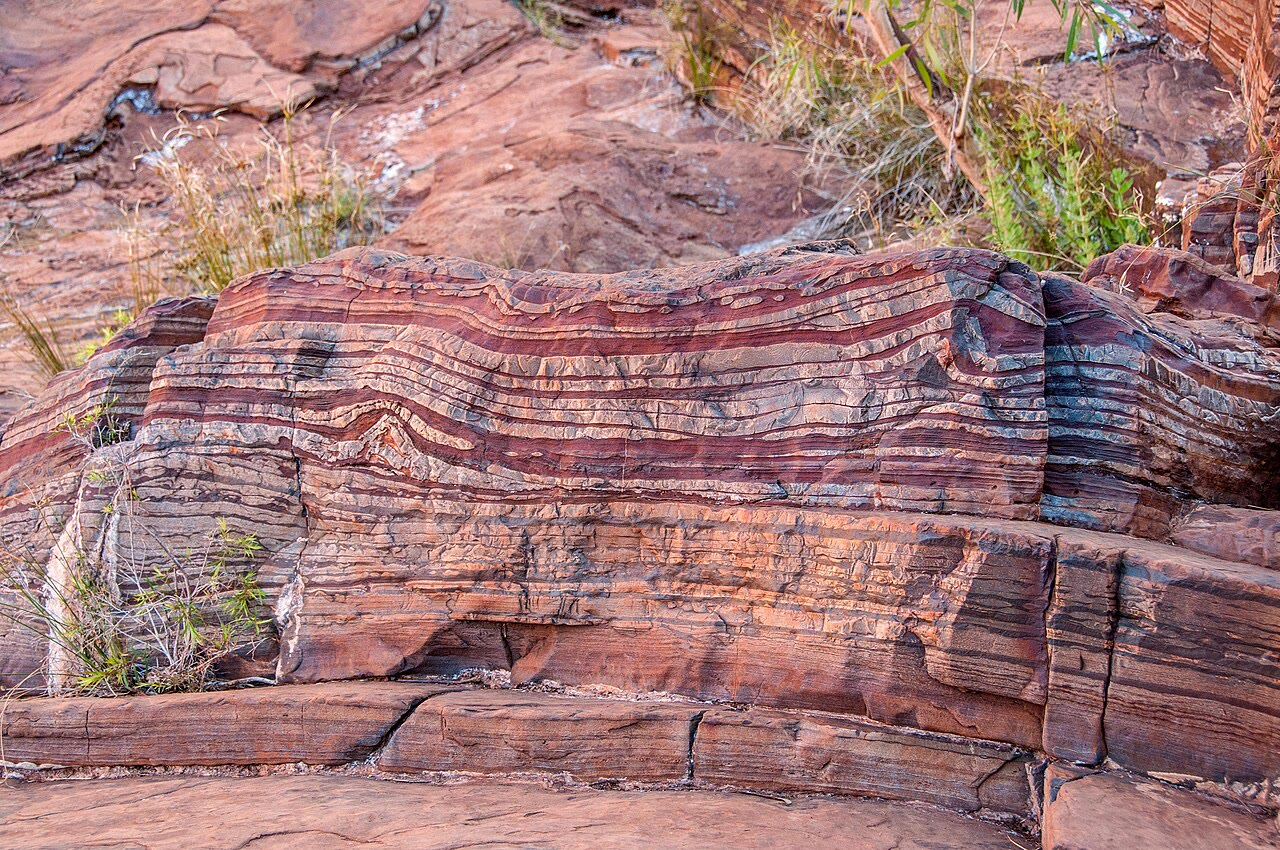
\includegraphics[width=0.72\linewidth]{images/book2/g12-dales-gorge-bif.jpg}

{\small \omterm{def:g12:early-earth:bif}{Formación de hierro bandeado} en las cascadas de Fortescue, garganta de
Dales, Parque Nacional de Karijini, Australia Occidental. Fotografía de Graeme
Churchard, CC~BY~2.0 (Wikimedia Commons).}
\end{omfigure}

\begin{recall}
La Tierra tiene 4540 millones de años (el \cref{ch:g12:age-of-the-earth}), y
los circones muestran que ya existía una corteza hace 4400 millones de años
(el \cref{ch:g12:continental-crust}). La \omterm{def:g10:habitable-planet:equilibrium-temperature}{temperatura de equilibrio} de un
planeta, $T_{\mathrm{eq}} = \left(S(1-A)/(4\sigma)\right)^{1/4}$, es de unos
\qty{255}{K} para la Tierra actual (el \cref{ch:g10:habitable-planet}). El
aire seco actual tiene un \qty{78}{\percent} de nitrógeno y un
\qty{21}{\percent} de oxígeno, y el dióxido de carbono y el metano son gases
de efecto invernadero; un elemento que capta oxígeno se oxida (los libros de
química). Las plantas, las algas y las cianobacterias fabrican su alimento por
fotosíntesis, que libera oxígeno (los libros de biología).
\end{recall}
% ledger: usgs:age-earth (Book 1 row), wilde01:zircon, earth:TSI, earth:albedo, air:N2, air:O2

\section{La Tierra joven}

La Tierra creció por acreción de cuerpos más pequeños. Unos 60 millones de
años después de que el sistema solar empezara a formarse, un cuerpo quizá del
tamaño de Marte chocó con ella, y el material lanzado al espacio formó la
Luna. La Tierra joven estaba caliente y todavía en parte fundida. Se enfrió y,
hace unos 4400 millones de años, ya tenía una corteza y un océano: los
circones de esa edad llevan la huella química del agua líquida.
% ledger: nasa:moon-formation, wilde01:zircon

\section{La atmósfera primitiva}

\begin{definition}[Desgasificación; atmósfera primitiva]\label{def:g12:early-earth:primitive-atmosphere}
La \emph{desgasificación}\index{desgasificacion@desgasificación} es la
liberación, por los volcanes y a través del suelo, de los gases disueltos en
el magma. La \emph{atmósfera primitiva}\index{atmosfera primitiva@atmósfera primitiva}
es la atmósfera de la Tierra antes de que los seres vivos la modificaran:
formada sobre todo por desgasificación, contenía nitrógeno, dióxido de carbono
y vapor de agua, más dióxido de carbono que hoy, y casi nada de oxígeno libre.
\end{definition}
% ledger: usgs:volcanic-gases (Book 1 row), holland06:stages (stage 1 anoxic), feulner12:fys (more carbon dioxide)

Los volcanes muestran todavía cómo se forma una atmósfera así: a medida que el
magma asciende y la presión baja, sus gases disueltos escapan, y el más
abundante, con mucho, es el vapor de agua, seguido del dióxido de carbono. El
nitrógeno y el dióxido de carbono, los gases que dominaban el aire primitivo,
siguen siendo hoy los principales gases volcánicos con nitrógeno y con
carbono. El vapor de agua se condensó y formó el océano. El oxígeno no llegaba
al \qty{0.001}{\percent} de su nivel en el aire actual.
% ledger: usgs:volcanic-gases (Book 1 row), pk02:anoxic

El Sol joven brillaba menos que hoy. A medida que transforma hidrógeno en
helio en su núcleo, el núcleo se contrae y se calienta, y la potencia del Sol
aumenta lentamente.

\begin{proposition}[La luminosidad del Sol joven]\label{prop:g12:early-earth:luminosity}
Si $t_\odot$ es la edad actual del Sol y $L_\odot$ su luminosidad actual, su
luminosidad cuando tenía $t$ años era
\[
  L(t) = \frac{L_\odot}{1 + \frac{2}{5}\left(1 - t/t_\odot\right)} .
\]
\end{proposition}
% ledger: gough81:luminosity, connelly12:cai

Esta aproximación de los modelos calculados del Sol se admite aquí. En el
nacimiento del Sol, $t = 0$, da $L = L_\odot/1.4 \approx 0.71\,L_\odot$: el
Sol joven era alrededor de un \qty{30}{\percent} menos brillante.

\begin{example}[La Tierra hace cuatro mil millones de años]\label{ex:g12:early-earth:young-sun}
Toma $t_\odot = 4.567$ miles de millones de años. Hace cuatro mil millones de
años, el Sol tenía 0.567 miles de millones de años, así que $1 - t/t_\odot = 4/4.567 \approx 0.876$ y
$L \approx L_\odot/1.350 \approx 0.741\,L_\odot$. La luz solar que llegaba a
la Tierra era de $0.741 \times 1361 \approx \qty{1008}{W/m^2}$. Con el \omterm{def:g10:earth-energy-budget:albedo}{albedo}
actual, la \omterm{def:g10:habitable-planet:equilibrium-temperature}{temperatura de equilibrio} varía como la raíz cuarta de la luz
solar: $255 \times 0.741^{1/4} \approx 255 \times 0.928 \approx
\qty{237}{K}$, unos \qty{-36}{\celsius}.
\end{example}
% values: L_4Ga 0.7406, S_4Ga 1007.9, Teq_today 255.1, Teq_4Ga 236.7 (early_earth.py)

\begin{omfigure}
\begin{tikzpicture}
\begin{axis}[omrecord, scale only axis, width=0.66\linewidth, height=4.6cm,
  xmin=0, xmax=4.6, ymin=225, ymax=295, x dir=reverse, axis y line*=left,
  xlabel={tiempo antes del presente (miles de millones de años)}, ylabel={temperatura (K)},
  xtick={0,0.5,...,4.5}, x tick label style={/pgf/number format/.cd, fixed, precision=1}]
% computed in figdata/grade-12/early_earth.py; ledger: gough81:luminosity, earth:TSI, earth:albedo, earth:Tsurf
\addplot[omDef, line width=1.2pt] table[x=t_Ga, y=Teq] {figdata/out/grade-12-early_earth-sun.dat};
\addplot[omThm, densely dashed, domain=0:4.6, samples=2] {273.15};
\addplot[black!60, densely dotted, domain=0:4.6, samples=2] {288};
\coordinate (teq) at (axis cs:2.6,239);
\coordinate (frz) at (axis cs:2.3,274);
\coordinate (sfc) at (axis cs:2.3,289);
\end{axis}
\begin{axis}[omrecord, scale only axis, width=0.66\linewidth, height=4.6cm,
  xmin=0, xmax=4.6, ymin=0.65, ymax=1.05, x dir=reverse, axis y line*=right, axis x line=none,
  ylabel={luminosidad del Sol ($L_\odot$)}, ymajorgrids=false, xmajorgrids=false,
  y tick label style={/pgf/number format/.cd, fixed, fixed zerofill, precision=2}]
\addplot[omProp, line width=0.9pt, densely dashdotted] table[x=t_Ga, y=L] {figdata/out/grade-12-early_earth-sun.dat};
\coordinate (lum) at (axis cs:1.7,0.86);
\end{axis}
\node[font=\scriptsize, text=omDef, anchor=north] at (teq) {temperatura de equilibrio};
\node[font=\scriptsize, text=omThm, anchor=south] at (frz) {el agua se congela, \qty{273}{K}};
\node[font=\scriptsize, text=black!70, anchor=south] at (sfc) {superficie media hoy, \qty{288}{K}};
\node[font=\scriptsize, text=omProp, anchor=north west] at (lum) {luminosidad (escala derecha)};
\end{tikzpicture}

{\small El Sol joven débil: su luminosidad (escala de la derecha) y la
\omterm{def:g10:habitable-planet:equilibrium-temperature}{temperatura de equilibrio} de la Tierra con el \omterm{def:g10:earth-energy-budget:albedo}{albedo} actual (escala de la
izquierda), hasta el nacimiento del Sol. Calculado a partir de Gough (1981)
con la luz solar y el \omterm{def:g10:earth-energy-budget:albedo}{albedo} actuales.}
\end{omfigure}

\begin{definition}[Paradoja del Sol joven débil]\label{def:g12:early-earth:faint-young-sun}
La \emph{paradoja del Sol joven débil}\index{paradoja del Sol joven debil@paradoja del Sol joven débil}
es la contradicción entre el Sol menos brillante de los primeros miles de
millones de años de la Tierra, bajo el cual la Tierra, con la atmósfera
actual, se habría congelado, y las rocas, que muestran que había agua líquida.
\end{definition}
% ledger: feulner12:fys

El problema lo dieron a conocer ampliamente en 1972 Carl Sagan y George
Mullen, que propusieron como respuesta un efecto invernadero más fuerte. La
mayoría de las respuestas estudiadas desde entonces recurren a más gases de
efecto invernadero en la \omterm{def:g12:early-earth:primitive-atmosphere}{atmósfera primitiva}: mucho más dióxido de carbono que
hoy, metano producido por los primeros microbios, o ambos. En un cálculo
clásico, alrededor de una décima de bar de dióxido de carbono, con un poco de
metano, mantiene la Tierra joven tan caliente como hoy; sin el metano, hace
falta unas tres veces más. El problema aún no se considera resuelto.
% ledger: feulner12:fys

\section{La vida y el oxígeno}

El registro fósil de los \omterm{def:g12:early-earth:stromatolite}{estromatolitos} abarca casi \num{3500} millones de
años: están entre los indicios de vida más antiguos.

\begin{definition}[Estromatolito]\label{def:g12:early-earth:stromatolite}
Un \emph{estromatolito}\index{estromatolito} es un montículo estratificado
construido en aguas poco profundas por un tapete de microbios, sobre todo
cianobacterias, que atrapan y fijan granos de sedimento y hacen crecer
carbonato, capa sobre capa.
\end{definition}
% ledger: noffke13:stromatolites

En el Strelley Pool Chert del Pilbara, en Australia Occidental, se encuentran
\omterm{def:g12:early-earth:stromatolite}{estromatolitos} fósiles de \num{3430} millones de años. Hoy crecen
\omterm{def:g12:early-earth:stromatolite}{estromatolitos} vivos en el agua muy salada de Hamelin Pool, en la bahía
Shark, dos veces más salada que el agua de mar normal, donde son el ejemplo
moderno más conocido.
% ledger: allwood06:spc, noffke13:stromatolites, dbca:hamelin

\begin{omfigure}
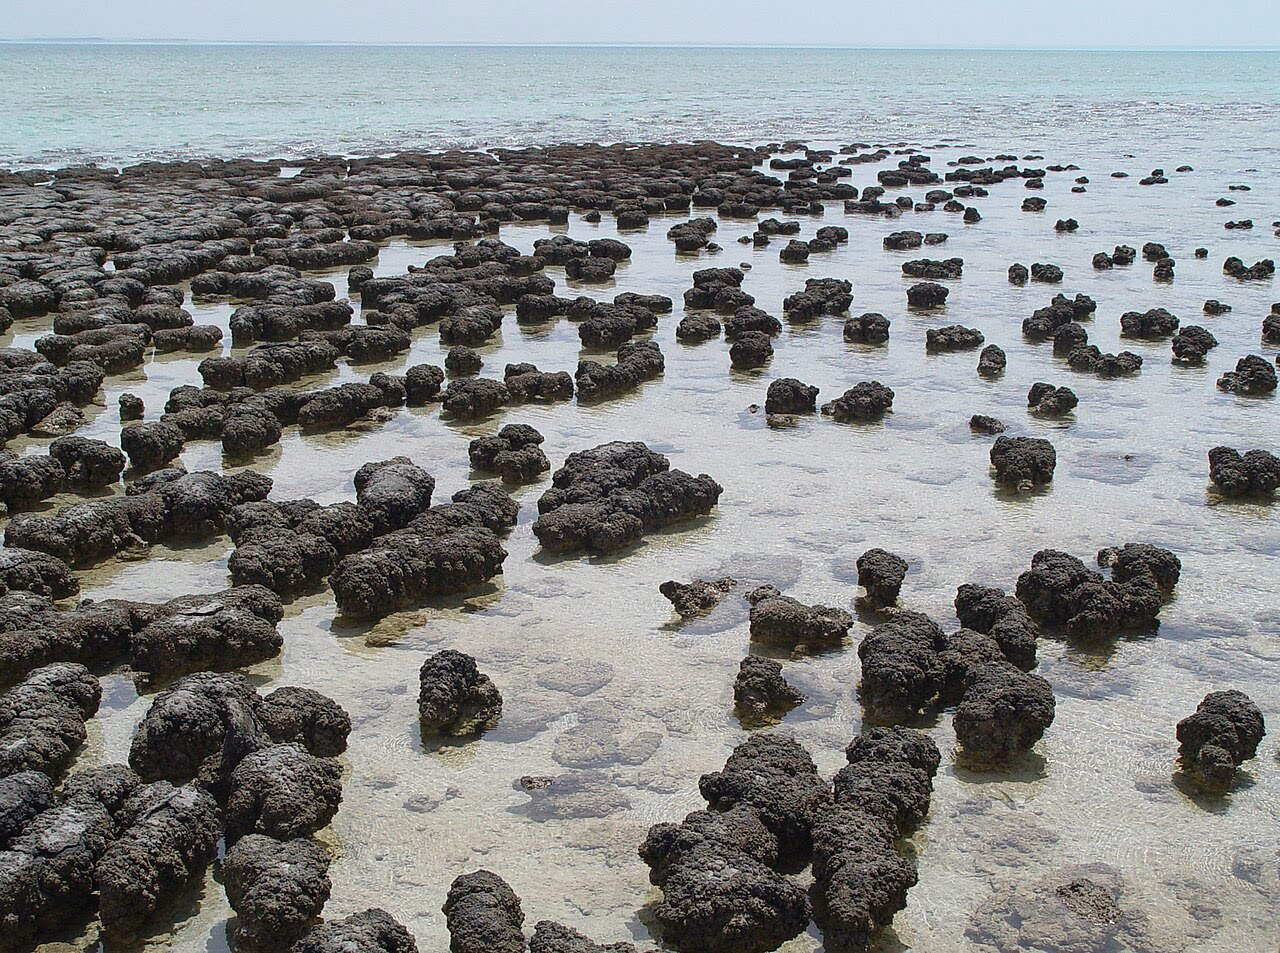
\includegraphics[width=0.6\linewidth]{images/book2/g12-shark-bay-stromatolites.jpg}

{\small \omterm{def:g12:early-earth:stromatolite}{Estromatolitos} vivos en Hamelin Pool, bahía Shark, Australia
Occidental. Fotografía de Paul Harrison, CC~BY-SA~3.0 (Wikimedia Commons).}
\end{omfigure}
% ledger: photo:g12-shark-bay

Las cianobacterias trajeron algo nuevo: una fotosíntesis que libera oxígeno.
Pero durante mucho tiempo el oxígeno que producían no permaneció en el aire.
Se consumía tan deprisa como se producía: por el hierro disuelto en el mar,
por el azufre y por el metano.

\section{El ascenso del oxígeno}

Antes del oxígeno, el hierro podía viajar disuelto en el agua de mar como ion
\ce{Fe^2+}. El oxígeno lo transforma en hierro(III), que no se disuelve: cae
al fondo como un sedimento oxidado.

\begin{proposition}[El hierro capta oxígeno]\label{prop:g12:early-earth:iron}
El hierro(II) disuelto se oxida por el oxígeno en el agua a hidróxido de
hierro(III), que precipita:
\[
  \ce{4Fe^2+ + O2 + 10H2O -> 4Fe(OH)3 + 8H+} .
\]
Cada molécula de oxígeno elimina cuatro iones de hierro disuelto; mientras
quede hierro disuelto, el oxígeno producido se consume.
\end{proposition}
% ledger: earle:bif (ferrous iron oxidised to insoluble ferric iron)

\begin{proof}
Comprueba el ajuste. Hierro: 4 en cada lado. Oxígeno: $2 + 10 = 12$ a la
izquierda, $4 \times 3 = 12$ a la derecha. Hidrógeno: $20$ a la izquierda,
$4 \times 3 + 8 =
20$ a la derecha. Carga: $4 \times (+2) = +8$ a la
izquierda, $8 \times (+1) =
+8$ a la derecha.
\end{proof}

\begin{definition}[Formación de hierro bandeado]\label{def:g12:early-earth:bif}
Una \emph{formación de hierro bandeado}\index{formacion de hierro bandeado@formación de hierro bandeado}
es una roca sedimentaria de finas capas alternas de óxidos de hierro, como la
hematites, y de sílex, una sílice de grano fino pobre en hierro. Casi todas
tienen más de 1800 millones de años.
\end{definition}
% ledger: earle:bif, holland06:stages

Las \omterm{def:g12:early-earth:bif}{formaciones de hierro bandeado} necesitan dos aguas a la vez: un \omterm{def:g10:layered-ocean:thermocline}{océano
profundo} sin oxígeno, que lleva hierro disuelto, y un mar poco profundo e
iluminado por el sol donde las cianobacterias producen oxígeno y el hierro
precipita. Son comunes en las rocas de 2400 a 1800 millones de años, y las de
los montes Hamersley son aún más antiguas. Las \omterm{def:g12:early-earth:bif}{formaciones de hierro bandeado}
son una mena de hierro corriente.
% ledger: earle:bif, holland06:stages (Archean BIF, Hamersley), dbca:karijini

\begin{omfigure}
\begin{tikzpicture}[x=1cm, y=1cm, font=\scriptsize]
  % sea and floor
  \fill[omSea] (0,0) rectangle (11,4);
  \fill[omSea!45!white] (0,2.9) rectangle (11,4);
  \draw[omDef!60, line width=0.4pt, densely dashed] (0,2.9) -- (11,2.9);
  \node[anchor=north east, text=omDef] at (10.9,3.95) {agua superficial iluminada};
  \node[anchor=south east, text=omDef, align=right] at (10.9,0.12) {agua profunda\\sin oxígeno,\\rica en \ce{Fe^2+}};
  % floor with layers
  \foreach \i/\c in {0/red!55!black, 1/black!20, 2/red!55!black, 3/black!20, 4/red!55!black, 5/black!20} {
    \fill[\c] (0,-0.12*\i) rectangle (11,-0.12*\i-0.12);
  }
  \draw[black!60] (0,0) -- (11,0);
  \node[anchor=west] at (11.1,-0.12) {óxido de hierro};
  \node[anchor=west] at (11.1,-0.36) {sílex};
  \draw[black!50, line width=0.3pt] (11.05,-0.06) -- (10.6,-0.06);
  \draw[black!50, line width=0.3pt] (11.05,-0.30) -- (10.6,-0.30);
  % upwelling iron
  \foreach \x in {0.5,1.0,1.5} {
    \draw[-{Stealth}, omDef, line width=0.8pt] (\x,0.4) .. controls (\x+0.4,1.5) and (\x+0.6,2.2) .. (\x+0.9,2.85);
  }
  \node[text=omDef, anchor=west] at (2.3,1.3) {el \ce{Fe^2+} sube};
  % cyanobacteria and oxygen
  \foreach \x in {3.8,4.4,5.0,5.6,6.2} {\fill[green!45!black] (\x,3.35) circle (0.07);}
  \node[anchor=south, text=green!35!black] at (5.0,3.47) {las cianobacterias producen \ce{O2}};
  % reaction
  \node[draw=black!40, fill=white, rounded corners=2pt, inner sep=2pt] at (5.4,2.45) {\ce{4Fe^2+ + O2 + 10H2O -> 4Fe(OH)3 + 8H+}};
  % falling rust
  \foreach \x/\y in {4.6/1.9, 5.0/1.5, 5.5/1.8, 5.9/1.2, 4.3/1.1, 5.2/0.7, 6.1/0.6} {\fill[red!60!black] (\x,\y) circle (0.06);}
  \draw[-{Stealth}, red!60!black, line width=0.6pt] (6.6,2.1) -- (6.6,0.25);
  \node[anchor=west, text=red!60!black, align=left] at (6.7,1.75) {el hierro(III) se deposita\\en una capa oxidada};
\end{tikzpicture}

{\small Cómo se forma una \omterm{def:g12:early-earth:bif}{formación de hierro bandeado} (esquema, sin escala):
el hierro disuelto en el agua profunda, que no contiene oxígeno, asciende
hasta el mar iluminado, donde el oxígeno producido por las cianobacterias lo
transforma en hierro(III), que se deposita. Las capas ricas en hierro alternan
con capas de sílex.}
\end{omfigure}

Después, el oxígeno empezó a permanecer en el aire.

\begin{definition}[Gran Evento de Oxidación]\label{def:g12:early-earth:goe}
El \emph{Gran Evento de Oxidación}\index{Gran Evento de Oxidacion@Gran Evento de Oxidación}
es el intervalo, de hace unos \num{2.46} a unos \num{2.06}~mil millones de
años, durante el cual el oxígeno libre se acumuló por primera vez en la
atmósfera de la Tierra y en los mares poco profundos, hasta alcanzar quizá una
décima parte de su nivel actual.
\end{definition}
% ledger: gumsley17:goe, holland06:stages (0.02-0.04 atm, about a tenth of 0.21)

Las pruebas están en las rocas. Algunos minerales, entre ellos la pirita y la
uraninita, son destruidos por el oxígeno; sin embargo, se encuentran granos de
ellos, rodados por los ríos, en sedimentos antiguos, y faltan los granos de
pirita en los depositados después del ascenso del oxígeno. Los isótopos del
azufre de las rocas de más de unos 2450 millones de años llevan una firma que
solo puede dejar un aire con menos de una cienmilésima del oxígeno actual;
hace 2090 millones de años ya ha desaparecido. Y en tierra firme aparecieron
las \omterm{def:g12:early-earth:red-beds}{capas rojas}.
% ledger: kasting25:indicators, pk02:anoxic, farquhar00:sulfur

\begin{definition}[Capas rojas]\label{def:g12:early-earth:red-beds}
Las \emph{capas rojas}\index{capas rojas} son rocas sedimentarias
---areniscas, limolitas, lutitas--- coloreadas de rojo por un recubrimiento de
óxido de hierro(III), la hematites, sobre sus granos. Solo se forman donde hay
oxígeno suficiente para oxidar el hierro.
\end{definition}
% ledger: kasting25:indicators (redbeds an oxygen indicator)

\begin{omfigure}
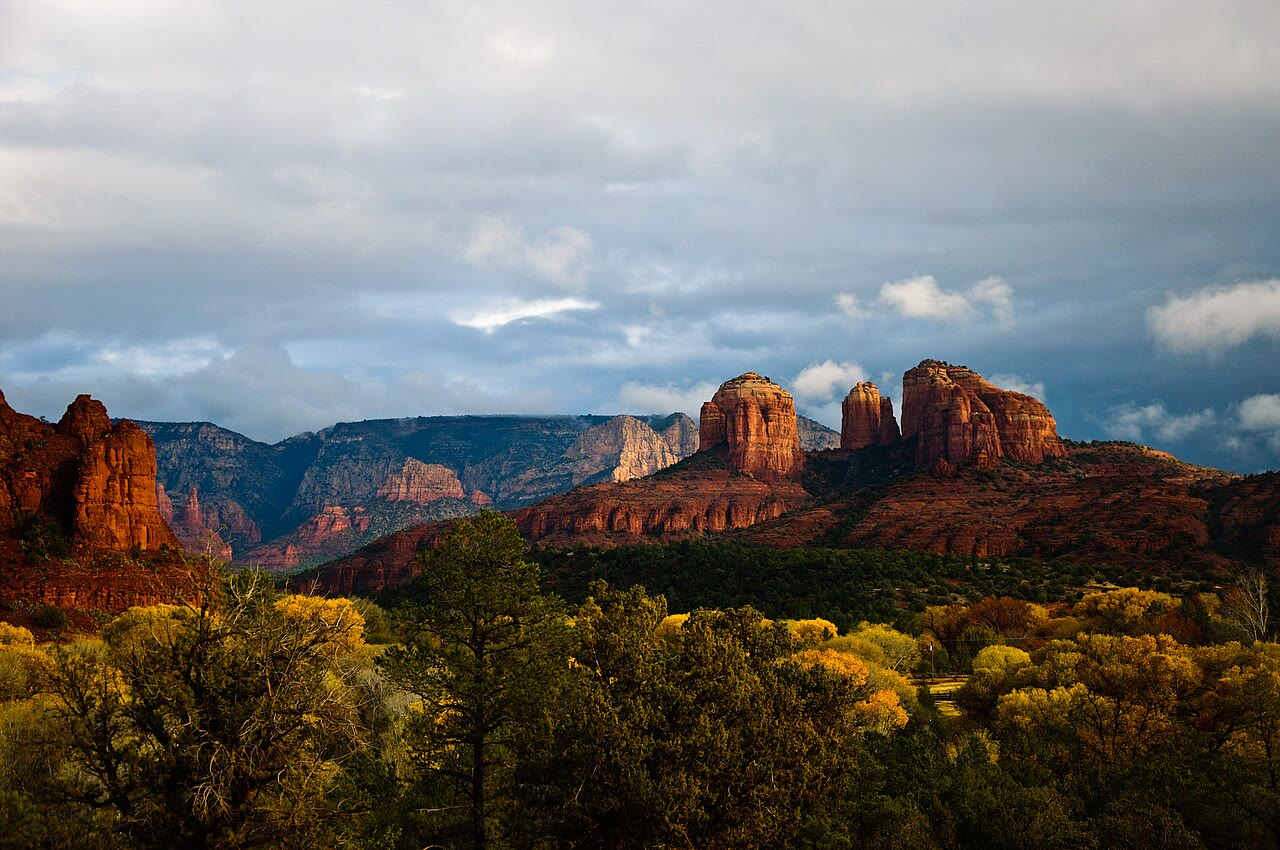
\includegraphics[width=0.66\linewidth]{images/book2/g12-sedona-red-beds.jpg}

{\small \omterm{def:g12:early-earth:red-beds}{Capas rojas}: Cathedral Rock, cerca de Sedona, Arizona, formada por
areniscas rojas del Pérmico. Fotografía de Wendy from Pennsylvania,
CC~BY-SA~2.0 (Wikimedia Commons).}
\end{omfigure}
% ledger: photo:g12-sedona, azgs:cathedral (Permian Schnebly Hill Sandstone)

La \omterm{def:g12:early-earth:bif}{formación de hierro bandeado} prácticamente cesó después de hace 1800
millones de años: para entonces, también el \omterm{def:g10:layered-ocean:thermocline}{océano profundo} tenía oxígeno
suficiente para dejar de transportar hierro. Durante los mil millones de años
siguientes, el oxígeno cambió poco; a partir de hace 850 millones de años
volvió a acumularse, hacia el \qty{21}{\percent} actual.
% ledger: earle:bif, holland06:stages

\begin{method}[Leer una línea del tiempo geológica]\label{met:g12:early-earth:timeline}
\begin{enumerate}
  \item Averigua en qué sentido corre el tiempo en el eje, y su unidad
        (millones o miles de millones de años antes del presente).
  \item Localiza los eones en la banda de colores y lee sus límites.
  \item Para cada suceso, lee su fecha, o el intervalo en que ocurrió, y di
        qué registro lo data (un mineral, un fósil, una roca).
  \item Calcula las duraciones por resta, y compáralas con la \omterm{def:g12:age-of-the-earth:age}{edad de la
        Tierra}.
  \item Comprueba el orden: un efecto no debe preceder a su causa.
\end{enumerate}
\end{method}

\begin{omfigure}
\begin{tikzpicture}
\begin{axis}[omrecord, width=0.82\linewidth, height=6.2cm, ymode=log, xmin=0, xmax=4.6, ymin=1e-7, ymax=5,
  x dir=reverse, xlabel={tiempo antes del presente (miles de millones de años)}, ylabel={oxígeno en el aire (hoy $=1$)},
  xtick={0,0.5,...,4.5}, x tick label style={/pgf/number format/.cd, fixed, precision=1},
  ytick={1e-6,1e-4,1e-2,1}, ymajorgrids=true, xmajorgrids=false, clip=false]
% computed in figdata/grade-12/early_earth.py (schematic through the sourced bounds); ledger: holland06:stages, pk02:anoxic, gumsley17:goe, ics:base.Hadean, ics:base.Archean, ics:base.Proterozoic, ics:base.Paleozoic
\fill[omThm!12] (axis cs:2.46,1e-7) rectangle (axis cs:2.06,5);
\addplot[black, line width=1.2pt] table[x=t_Ga, y=pal] {figdata/out/grade-12-early_earth-oxygen.dat};
% eon band (ICS colours), below the axis
\fill[icsHadean] (axis cs:4.567,1.5e-7) rectangle (axis cs:4.031,4e-7);
\fill[icsArchean] (axis cs:4.031,1.5e-7) rectangle (axis cs:2.5,4e-7);
\fill[icsProterozoic] (axis cs:2.5,1.5e-7) rectangle (axis cs:0.5388,4e-7);
\fill[icsPhanerozoic] (axis cs:0.5388,1.5e-7) rectangle (axis cs:0,4e-7);
\node[font=\tiny, text=white] at (axis cs:4.30,2.45e-7) {Hádico};
\node[font=\tiny, text=white] at (axis cs:3.27,2.45e-7) {Arcaico};
\node[font=\tiny, text=white] at (axis cs:1.52,2.45e-7) {Proterozoico};
% events
\draw[omDef, line width=0.6pt] (axis cs:4.4,4e-7) -- (axis cs:4.4,3e-3);
\node[font=\scriptsize, text=omDef, anchor=south west] at (axis cs:4.4,3e-3) {circones, agua};
\draw[omMeth, line width=0.6pt] (axis cs:3.43,4e-7) -- (axis cs:3.43,1.2e-6);
\node[font=\scriptsize, text=omMeth, anchor=south] at (axis cs:3.43,1.2e-6) {primeros estromatolitos};
\draw[red!60!black, line width=3pt] (axis cs:2.4,3e-6) -- (axis cs:1.8,3e-6);
\node[font=\scriptsize, text=red!60!black, anchor=north] at (axis cs:2.16,2.4e-6) {formaciones de hierro bandeado};
\node[font=\scriptsize, text=omThm, anchor=south, align=center] at (axis cs:2.26,1.2) {Gran Evento\\de Oxidación};
\node[font=\scriptsize, anchor=south] at (axis cs:3.2,1.3e-5) {menos de $10^{-5}$ del actual};
\node[font=\scriptsize, anchor=south] at (axis cs:1.4,0.12) {alrededor de una décima};
\end{axis}
\end{tikzpicture}

{\small El oxígeno del aire a lo largo del tiempo (esquema, escala
logarítmica): la curva une los límites medidos y oculta los altibajos del
registro real. El intervalo sombreado es el \omterm{def:g12:early-earth:goe}{Gran Evento de Oxidación}; la barra
roja marca la época en que las \omterm{def:g12:early-earth:bif}{formaciones de hierro bandeado} eran comunes,
de hace 2400 a 1800 millones de años. Eones según la Tabla
Cronoestratigráfica Internacional.}
\end{omfigure}

\section{Ejercicios}

\begin{exercise}[$\star$]\label{exo:g12:early-earth:1}
Da la palabra: (a) la liberación de los gases disueltos en el magma; (b) un
montículo estratificado construido por un tapete microbiano; (c) una roca de
capas alternas de óxido de hierro y de sílex; (d) rocas sedimentarias
coloreadas por la hematites; (e) el intervalo en que el oxígeno se acumuló por
primera vez en el aire.
\end{exercise}

\begin{exercise}[$\star$]\label{exo:g12:early-earth:2}
Ordena, de la más antigua a la más reciente: el final de la mayoría de las
\omterm{def:g12:early-earth:bif}{formaciones de hierro bandeado}; los primeros \omterm{def:g12:early-earth:stromatolite}{estromatolitos} del Pilbara; los
circones que muestran agua líquida; las \omterm{def:g12:early-earth:bif}{formaciones de hierro bandeado} de
Hamersley; el final del \omterm{def:g12:early-earth:goe}{Gran Evento de Oxidación}.
\end{exercise}

\begin{exercise}[$\star$]\label{exo:g12:early-earth:3}
Con la ley de la luminosidad, calcula la luminosidad del Sol en su
nacimiento, como fracción de la actual. ¿En qué porcentaje era menos brillante?
\end{exercise}

\begin{exercise}[$\star$]\label{exo:g12:early-earth:4}
Se encuentran granos de pirita rodados por los ríos en sedimentos antiguos,
pero no en los depositados después del ascenso del oxígeno. ¿Qué te dice esto
sobre el aire en la época de los sedimentos antiguos? ¿Por qué?
\end{exercise}

\begin{exercise}[$\star$]\label{exo:g12:early-earth:5}
Nombra los dos gases más abundantes que liberan los volcanes, y di qué fue de
cada uno en la Tierra joven.
\end{exercise}

\begin{exercise}[$\star\star$]\label{exo:g12:early-earth:6}
Calcula la luminosidad del Sol y la \omterm{def:g10:habitable-planet:equilibrium-temperature}{temperatura de equilibrio} de la Tierra
(hoy \qty{255}{K}, con el mismo \omterm{def:g10:earth-energy-budget:albedo}{albedo}) hace 3000 millones de años y hace 2450
millones de años, tomando $t_\odot = 4.567$ miles de millones de años.
\end{exercise}

\begin{exercise}[$\star\star$]\label{exo:g12:early-earth:7}
¿Cuánto oxígeno hace falta para precipitar \qty{1}{kg} de hierro disuelto en
forma de hidróxido de hierro(III)? (Masas molares: hierro
\qty{55.85}{g/mol}, oxígeno \qty{16.00}{g/mol}.)
\end{exercise}

\begin{exercise}[$\star\star$]\label{exo:g12:early-earth:8}
Con la línea del tiempo, (1) ¿cuánto duró el \omterm{def:g12:early-earth:goe}{Gran Evento de Oxidación}? (2)
¿Durante qué fracción de la historia de la Tierra casi no hubo oxígeno en el
aire? (3) ¿Cuánto tiempo después de los primeros \omterm{def:g12:early-earth:stromatolite}{estromatolitos} empezó a
acumularse el oxígeno?
\end{exercise}

\begin{exercise}[$\star\star$]\label{exo:g12:early-earth:9}
Una \omterm{def:g12:early-earth:bif}{formación de hierro bandeado} y una capa roja contienen las dos óxido de
hierro(III). ¿Qué te dice cada una sobre el oxígeno, y dónde: en el mar
profundo, en el mar poco profundo, en el aire?
\end{exercise}

\begin{exercise}[$\star\star$]\label{exo:g12:early-earth:10}
¿Dónde pueden verse hoy \omterm{def:g12:early-earth:stromatolite}{estromatolitos} vivos? ¿Qué tiene de especial el agua
de ese lugar, y cómo crece un \omterm{def:g12:early-earth:stromatolite}{estromatolito} capa sobre capa?
\end{exercise}

\begin{exercise}[$\star\star$]\label{exo:g12:early-earth:11}
El oxígeno es el \qty{21}{\percent} del aire actual. ¿Qué porcentaje era
cuando estaba (1) a una cienmilésima del nivel actual; (2) a una décima del
nivel actual?
\end{exercise}

\begin{exercise}[$\star\star\star$]\label{exo:g12:early-earth:12}
Hace cuatro mil millones de años, ¿qué \omterm{def:g10:earth-energy-budget:albedo}{albedo} habría dado a la Tierra la
\omterm{def:g10:habitable-planet:equilibrium-temperature}{temperatura de equilibrio} actual, \qty{255}{K}, bajo el Sol joven ($L = 0.741\,L_\odot$,
\omterm{def:g10:earth-energy-budget:albedo}{albedo} actual 0.294)? ¿Es probable que un planeta con un océano, nubes y algo
de hielo fuera tan oscuro? ¿Cuál es la otra salida?
\end{exercise}

\begin{exercise}[$\star\star\star$]\label{exo:g12:early-earth:13}
Hoy, el efecto invernadero calienta la superficie de la Tierra de 255 a
\qty{288}{K}. Hace cuatro mil millones de años, la \omterm{def:g10:habitable-planet:equilibrium-temperature}{temperatura de equilibrio}
era de unos \qty{237}{K}. (1) ¿Cuántos kelvins de calentamiento por efecto
invernadero hacían falta entonces para llegar a \qty{273}{K}? ¿Y para llegar
a \qty{288}{K}? (2) Compáralo con el actual. (3) Un cálculo clásico necesita
alrededor de \qty{0.1}{bar} de dióxido de carbono, con un poco de metano;
compáralo con la presión de toda la atmósfera actual, de alrededor de
\qty{1}{bar}.
\end{exercise}

\begin{exercise}[$\star\star\star$]\label{exo:g12:early-earth:14}
Una firma especial de los isótopos del azufre solo puede formarse, y
conservarse en los sedimentos, cuando el aire contiene menos de $10^{-5}$ del
oxígeno actual. Se encuentra en las rocas de más de 2450 millones de años, y
no en las de menos de 2090 millones de años. (1) ¿Qué concluyes sobre el
oxígeno antes de hace 2450 millones de años? ¿Y después de hace 2090
millones? (2) ¿Es coherente con las fechas del \omterm{def:g12:early-earth:goe}{Gran Evento de Oxidación}?
\end{exercise}

\begin{exercise}[$\star\star\star$]\label{exo:g12:early-earth:15}
El impacto que formó la Luna ocurrió unos 60 millones de años después de que
el sistema solar empezara a formarse, lo que los primeros sólidos datan en
hace 4567 millones de años. (1) ¿Hacia cuándo ocurrió el impacto? (2) Los
circones más antiguos tienen \num{4404} millones de años. ¿Como máximo cuánto
tiempo después del impacto tenía ya la Tierra una corteza sólida y agua
líquida?
\end{exercise}
% ledger: nasa:moon-formation, connelly12:cai, wilde01:4404

\begin{problem}[{Problema de fin de semana --- El Sol joven débil}]
\label{pb:g12:early-earth:1}
% ledger: gough81:luminosity, connelly12:cai, earth:TSI, earth:albedo, earth:Tsurf, feulner12:fys, allwood06:spc, dbca:karijini, wilde01:zircon
% values (early_earth.py): L_4Ga 0.7406, S_4Ga 1007.9, Teq_today 255.1, Teq_4Ga 236.7, albedo_needed 0.047
El Sol tiene \num{4.567}~mil millones de años. Su luminosidad cuando tenía
$t$ años era $L(t) = L_\odot/\bigl(1 + \tfrac25 (1 - t/t_\odot)\bigr)$. Hoy,
la Tierra recibe \qty{1361}{W/m^2} de luz solar, refleja una fracción 0.294
de ella y tiene una \omterm{def:g10:habitable-planet:equilibrium-temperature}{temperatura de equilibrio} de \qty{255}{K}; su temperatura
media en superficie es de \qty{288}{K}.

\medskip
\noindent\textbf{Parte I --- El Sol hace cuatro mil millones de años.}
\begin{enumerate}
  \item ¿Qué edad tenía el Sol hace cuatro mil millones de años?
  \item Calcula $1 - t/t_\odot$ en ese momento.
  \item Calcula su luminosidad como fracción de la actual.
  \item ¿Qué luz solar recibía la Tierra, en \unit{W/m^2}?
  \item ¿En qué porcentaje era el Sol menos brillante que hoy?
\end{enumerate}

\medskip
\noindent\textbf{Parte II --- La temperatura de equilibrio.}
\begin{enumerate}[resume]
  \item Escribe la \omterm{def:g10:habitable-planet:equilibrium-temperature}{temperatura de equilibrio} en función de la luz solar $S$.
  \item Demuestra que, con el mismo \omterm{def:g10:earth-energy-budget:albedo}{albedo}, la temperatura varía como
        $S^{1/4}$.
  \item Calcula $0.741^{1/4}$.
  \item Calcula la \omterm{def:g10:habitable-planet:equilibrium-temperature}{temperatura de equilibrio} hace cuatro mil millones de años.
  \item Conviértela a grados Celsius.
\end{enumerate}

\medskip
\noindent\textbf{Parte III --- Pruebas de agua líquida.}
\begin{enumerate}[resume]
  \item ¿Qué muestran los circones de 4400 millones de años?
  \item ¿En qué tipo de agua crecieron los \omterm{def:g12:early-earth:stromatolite}{estromatolitos} del Pilbara, de
        \num{3430} millones de años?
  \item ¿Qué rocas de los montes Hamersley, depositadas en el mar hace más de
        2500 millones de años, necesitan agua líquida?
  \item Sin efecto invernadero, ¿se habría congelado el océano hace cuatro mil
        millones de años? ¿Por qué?
  \item Enuncia la contradicción que esto revela, y da su nombre.
\end{enumerate}

\medskip
\noindent\textbf{Parte IV --- El calentamiento por efecto invernadero necesario.}
\begin{enumerate}[resume]
  \item ¿Cuántos kelvins añade el efecto invernadero actual?
  \item ¿Cuántos hacían falta hace cuatro mil millones de años para mantener
        la superficie media por encima de \qty{273}{K}?
  \item ¿Qué \omterm{def:g10:earth-energy-budget:albedo}{albedo} habría dado \qty{255}{K} sin ningún efecto invernadero
        adicional? ¿Es verosímil?
  \item ¿Qué gas se cree que aportó la mayor parte del calentamiento
        adicional, y qué otro gas pudo ayudar?
  \item En resumen: ¿cuál era la \omterm{def:g10:habitable-planet:equilibrium-temperature}{temperatura de equilibrio} de la Tierra hace
        cuatro mil millones de años?
\end{enumerate}
\end{problem}
